\subsection{Linear finite element in 2D as a 2-depth ReLU DNN}\label{sec:2DFEMandDNN}
In this section, we will present our unexpected discovery pertaining to the
expressive power of ReLU DNNs, which derived from our investigation into ReLU DNNs 
in relation to hierarchical basis methods.

We have
$$
s(x) = x^2, \quad m(x,y) = xy,
$$
and 
$I_{\ell}$ means the interpolation on 1D and $\Pi_\ell$ means interpolation
on $[0,1]^2$ with mesh size $2^{-\ell}$.

In terms of the approximation of ReLU DNNs for $x^2$,
the most critical point is that
\begin{equation}\label{key}
	(I_{\ell} - I_{\ell-1})s(x) = -h_\ell^2\sum_{i\in \mathcal I_\ell}\phi_{\ell,i}(x) = -h_\ell^2g_\ell(x) \in {\mathcal N}_\ell^3
\end{equation}
for all $x\in \mathbb{R}$. Thus, a key question arises:
\begin{quote}
	Is there composition structure for $(\Pi_\ell - \Pi_{\ell-1})m (x, y)$?
\end{quote}

We have the following 
corollary for the explicit formula for $(\Pi_\ell- \Pi_{\ell-1})m$ on $[-1,1]^2$.
\begin{corollary}
	For any $(x,y) \in [-1,1]^2$, we have
	\begin{equation}\label{eq:Pi-Pi}
		\begin{aligned}
			&(\Pi_\ell- \Pi_{\ell-1})m (x,y) \\
			&= m_{\ell+2}(x,y) - m_{\ell+1}(x,y)  \\
			&= 2h^2_{\ell+1}\left(g_{\ell+1}\left(\frac{|x|}{2}\right)+g_{\ell+1}\left(\frac{|y|}{2}\right)-g_{\ell+1}\left(\frac{|x+y|}{2}\right)\right).
		\end{aligned}
	\end{equation}
	This means that $\psi_\ell \in \widehat{{\mathcal N}}_{3(\ell+2)}^3$ where $\psi_\ell = (\Pi_\ell- \Pi_{\ell-1})m$. Furthermore, 
	it is worth noting that we can actually have $\psi_\ell \in {\mathcal N}_{\ell+2}^9$ since $g_{\ell+1}(\frac{|x+y|}{2}) \in {\mathcal N}_{\ell+2}^3$.
\end{corollary}

By choosing a suitable scale, we have $\|h_{\ell}^{-2}(\Pi_\ell- \Pi_{\ell-1})m\|_{L^{\infty}([-1,1]^2)} = 1$. 
Fig.~\ref{fig:T2T3} shows function graphs of $h_2^{-2}(\Pi_2 - \Pi_{1})m$ and $h_{3}^{-2}(\Pi_3- \Pi_{2})m$ on $[0,1]^2$.
\begin{figure}[h!]
	\centering
	\begin{minipage}[t]{0.43\textwidth}
		\centering
		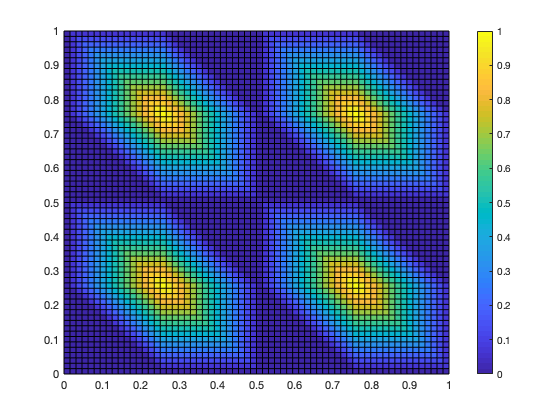
\includegraphics[width=\textwidth]{6DL/figures/4basis}
	\end{minipage}
	\begin{minipage}[t]{0.43\textwidth}
		\centering
		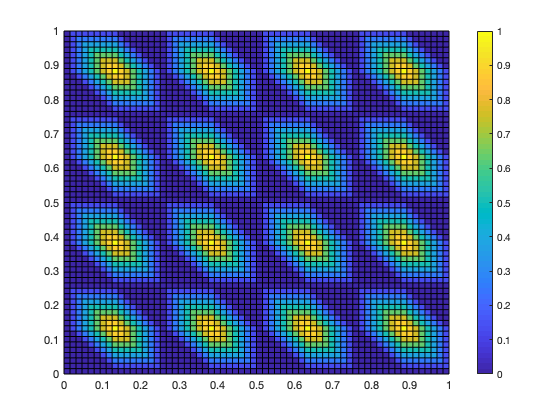
\includegraphics[width=\textwidth]{6DL/figures/16basis}
	\end{minipage}
	\caption{Functions of $h_{\ell}^{-2}(\Pi_\ell- \Pi_{\ell-1})m$ for $\ell = 2,3$ on $[0,1]^2$.}
	\label{fig:T2T3}
\end{figure}

These graphs and meshes of $(\Pi_\ell - \Pi_{\ell-1})m(x,y)$ give rise to a natural discussion about
the representation theorem of ReLU DNN for the basis function of the 2D linear finite element.
By taking $\ell=1$ with a suitable scale, we have
\begin{equation}\label{eq:varphi_1}
	4(\Pi_1- \Pi_{0})m (x,y) 
	= \frac{1}{2}\left(g_{2}\left(\frac{x}{2}\right)+g_2\left(\frac{y}{2}\right)-g_2\left(\frac{x+y}{2}\right)\right)
\end{equation}
for all $ (x,y) \in [0,1]^2$. 
Here, $4(\Pi_1- \Pi_{0})m (x,y)$ equals the basis function $\varphi(x,y)$ for the 
linear finite element (see left-hand graph of Fig.~\ref{fig:varphi_1}) 
on the uniform mesh on $[0,1]^2$ with mesh size $h_1=\frac{1}{2}$ (see right-hand graph of Fig.~\ref{fig:varphi_1}).
\begin{figure}[h!]
	\begin{minipage}[t]{0.43\linewidth}
		\centering
		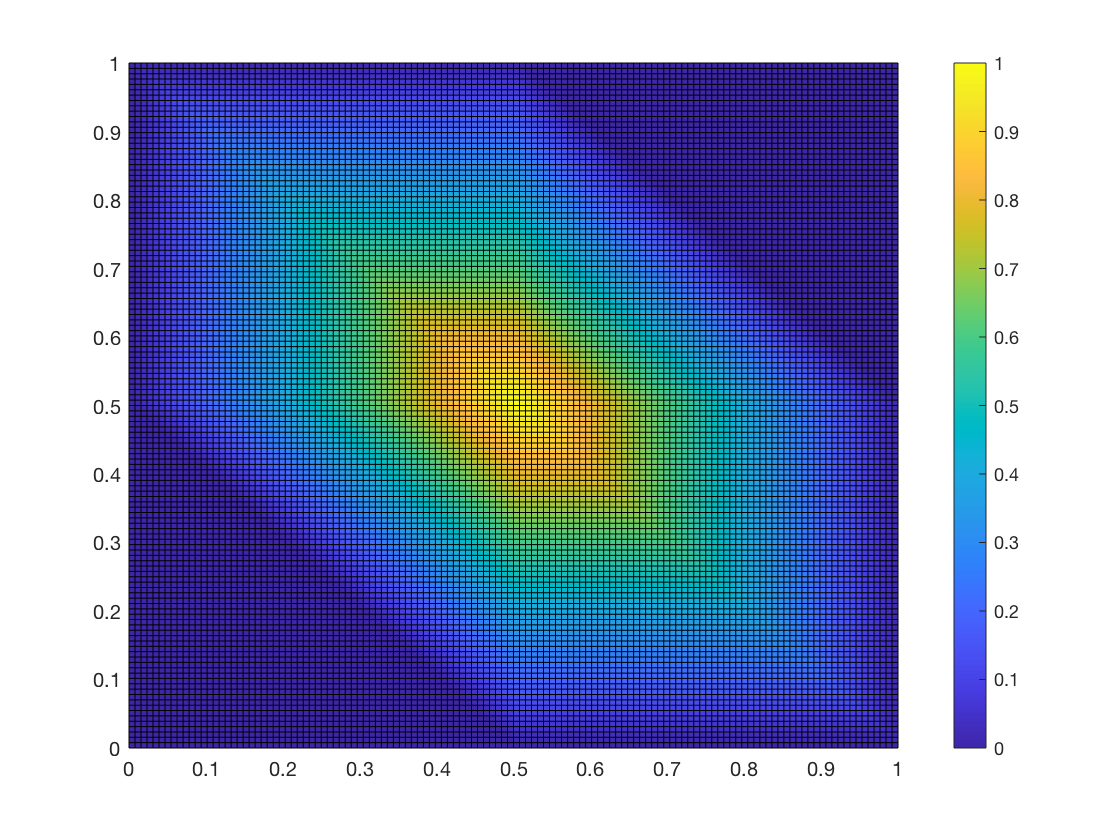
\includegraphics[width=\textwidth]{6DL/figures/varphi}
	\end{minipage}
	\begin{minipage}[t]{0.45\linewidth}
		\centering
		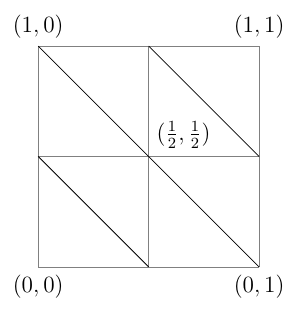
\includegraphics[scale=.5]{6DL/figures/2D_Basis}
		%		\begin{tikzpicture}[scale = 2 ]
		%		%\fill[green] (0,0) -- (0,2) -- (2,0) -- cycle;
		%		\draw[gray, step = 1cm] (0, 0) grid (2, 2);
		%		\node[anchor = north] at (0, 0) {$(0,0)$};
		%		%			\node[anchor = north] at (1,0) {$6$};
		%		\node[anchor = north] at (2,0) {$(0,1)$};
		%		%			\node[anchor = east] at (0,1) {$(\frac{1}{2},\frac{1}{2})$};
		%		\node[anchor = south west] at (1,1) {$(\frac{1}{2},\frac{1}{2})$};
		%		\node[anchor = south] at (0,2) {$(1,0)$};
		%		\node[anchor = south] at (2,2) {$(1,1)$};
		%		\draw(0,2) -- (2,0);
		%		\draw (0,1) -- (1,0);
		%		\draw (1,2) -- (2,1);
		%		\end{tikzpicture}
	\end{minipage}
	\caption{left: $\varphi(x,y)$ on $[0,1]^2$; right:  mesh for $\ell=1$ on $[0,1]^2$.}
	\label{fig:varphi_1}
\end{figure}
Without loss of generality, we can define $\varphi(x,y)$ globally as
\begin{equation}\label{key}
	\varphi(x,y) = \begin{cases}
		4(\Pi_1- \Pi_{0})m (x,y), \quad &(x,y) \in [0,1]^2, \\
		0, \quad &\text{others}.
	\end{cases}
\end{equation}
However, this representation,
\begin{equation}\label{eq:varphi_1-1}
	\varphi(x,y) = \frac{1}{2}\left(g_{2}\left(\frac{x}{2}\right)+g_2\left(\frac{y}{2}\right)-g_2\left(\frac{x+y}{2}\right)\right),
\end{equation}
holds only for $(x,y) \in [0,1]^2$. 
Related to this observation is the simple argument that 
\begin{equation}\label{key}
	\frac{1}{2}\left(g_{2}\left(\frac{x}{2}\right)+g_2\left(\frac{y}{2}\right)-g_2\left(\frac{x+y}{2}\right)\right) = \frac{1}{2} \neq 0
\end{equation}
if $(x,y) = (\frac{3}{2}, \frac{3}{2})$.
On the other hand, on the assumption that the identity in \eqref{eq:varphi_1-1} holds for all $(x,y) \in \mathbb{R}^2$, we can rewrite $g_2(x)$ as
\begin{equation}\label{eq:defg2_2}
	g_2(x) = \sum_{i=0}^4 \alpha_i {\rm ReLU}\left(x-\frac{i}{4}\right),
\end{equation}
for all $x\in \mathbb{R}$ where $(\alpha_0,\alpha_1,\cdots, \alpha_4) = (4, -8, 8, -8, 4)$ based on the relations between the linear finite element functions and ReLU DNNs on 1D~\cite{he2020relu}.
This means that $g_2 \in {\mathcal N}_{1}^5$ and $\varphi(x,y)$ can be represented by a ReLU DNN with only one hidden layer on the entire space $\mathbb{R}^2$.
However, this representation is contradictory to the theorem in~\cite{he2020relu} that the locally supported basis function of the 2D linear finite element cannot be represented globally by ReLU DNN  with just one hidden layer.

Given the global representation of $\varphi(x,y)$, \cite{he2019finite} constructs 
a ReLU DNN with four hidden layers to reproduce $\varphi(x,y)$ explicitly. 
Although \cite{arora2018understanding,he2020relu} show that
a two-hidden-layer ReLU DNN should be able to represent $\varphi(x,y)$ globally on $\mathbb{R}^2$,
the structure of network will be extremely complicated, as well as it requires a 
large number of neurons. Thus, to find a concise formula to 
reproduce $\varphi(x,y)$ on $\mathbb{R}^2$ directly becomes the focus of the inquiry.
Based on the discovery in \eqref{eq:varphi_1-1} and the properties of ReLU DNNs, 
we can construct a ReLU DNN function with two hidden layers to represent $\varphi(x,y)$. 
To simplify the statement of that result, let us first denote the following
${\rm ReLU1}(x)$ function:
\begin{equation}\label{eq:defReLU1}
	{\rm ReLU1}(x)  := {\rm ReLU}(x) - {\rm ReLU}(x-1) \in {\mathcal N}_1^2.
\end{equation}

\begin{lemma}
	The basis function $\varphi(x,y)$ is in  ${\mathcal N}_2^{15}$, more precisely, we have
	\begin{equation}\label{eq:b-DNN2}
		%\widehat b(x,y) := 
		{\varphi}(x,y) = \frac{1}{2}\left(g_{2}\left(\frac{{\rm ReLU1}(x)}{2}\right)+g_2\left(\frac{{\rm ReLU1}(y)}{2}\right)-g_2\left(\frac{{\rm ReLU1}(x)+{\rm ReLU1}(y)}{2}\right)\right)
	\end{equation}
	for all $(x,y) \in \mathbb{R}^2$. 
\end{lemma}
\begin{proof}
	According to the definition of $g_2(x)$ in \eqref{func:glinduction} (or \eqref{eq:defg2_2}) and ${\rm ReLU1}(x)$ in \eqref{eq:defReLU1},
	we have $ \varphi(x,y) \in {\mathcal N}_2^{15}$ and
	\begin{equation}\label{key}
		\varphi(x,y) = 0
	\end{equation}
	for any $(x,y) \notin [0,1]^2$ as ${\rm ReLU1}(x)$ and ${\rm ReLU1}(y)$ will equal to $0$ or $1$. 
	Then, \eqref{eq:b-DNN2} holds, given that ${\rm ReLU1}(x) = x$ and ${\rm ReLU1}(y) = y$ for $(x,y) \in [0,1]^2$.
\end{proof}

By employing the above lemma, we can construct the following theorem pertaining to the representation
of linear finite element functions by using ReLU DNNs with only two hidden layers on
two-dimensional space.
\begin{theorem}\label{thm:FEM-DNN}
	Assume $u_h$ is a two-dimensional linear finite element function, which can be written as
	\begin{equation}\label{key}
		u_h(x,y) = \sum_{i=1}^N \mu_i \varphi(T_i(x,y)), 
	\end{equation}
	where $T_i : \mathbb{R}^2 \mapsto \mathbb{R}^2$ is an affine mapping and $N$ denotes
	the number of degree of freedom. Then, $u_h(x)$ 
	can be reproduced globally by a ReLU DNN with only two hidden layers and $15N$ neurons
	at most for each layer, i.e., $u_h(x,y)  \in {\mathcal N}_2^{15N}$.
\end{theorem}
According to~\cite{arora2018understanding}, any d-dimensional continuous piecewise
linear function can be represented by ReLU DNNs with at most $\lceil \log_2(d+1) \rceil$ hidden layers.
However, the representation theory in \cite{arora2018understanding} requires an extremely complicated
construction by induction with a tremendously high number of neurons. On the other hand, \cite{he2020relu}
shows that ReLU DNNs with only one hidden layer cannot be used to represent general linear
finite element functions even on two-dimensional space. 
Thus, the focus inevitably turns to finding
a concise and explicit representation of linear finite element functions using ReLU DNNs with 
only two hidden layers on two-dimensional space. 
Here, Theorem~\ref{thm:FEM-DNN} provides the answer for any two-dimensional linear finite element functions on a uniform mesh or meshes, which can be obtained by adding affine mappings.